\section{User Documentation}
\textit{(This section is also part of the readme.md on the weekme-github repository)} \\
\\Using \textbf{WeekMe} you can plan your next week. Not more, not less. No bloated UI nor functions you will probably never use anyway. 
How does this \textbf{awesome application} work? Hopefully it's so intuitive that any explanation is unnecessary but just in case here we give you a short introduction.

\subsection{Account}
Like in most web apps you can sign up for an account, log in and out as well as change your password and email. And of course there is also a solution in case you forget your password. 
\begin{figure}[H] 
	\centering 
	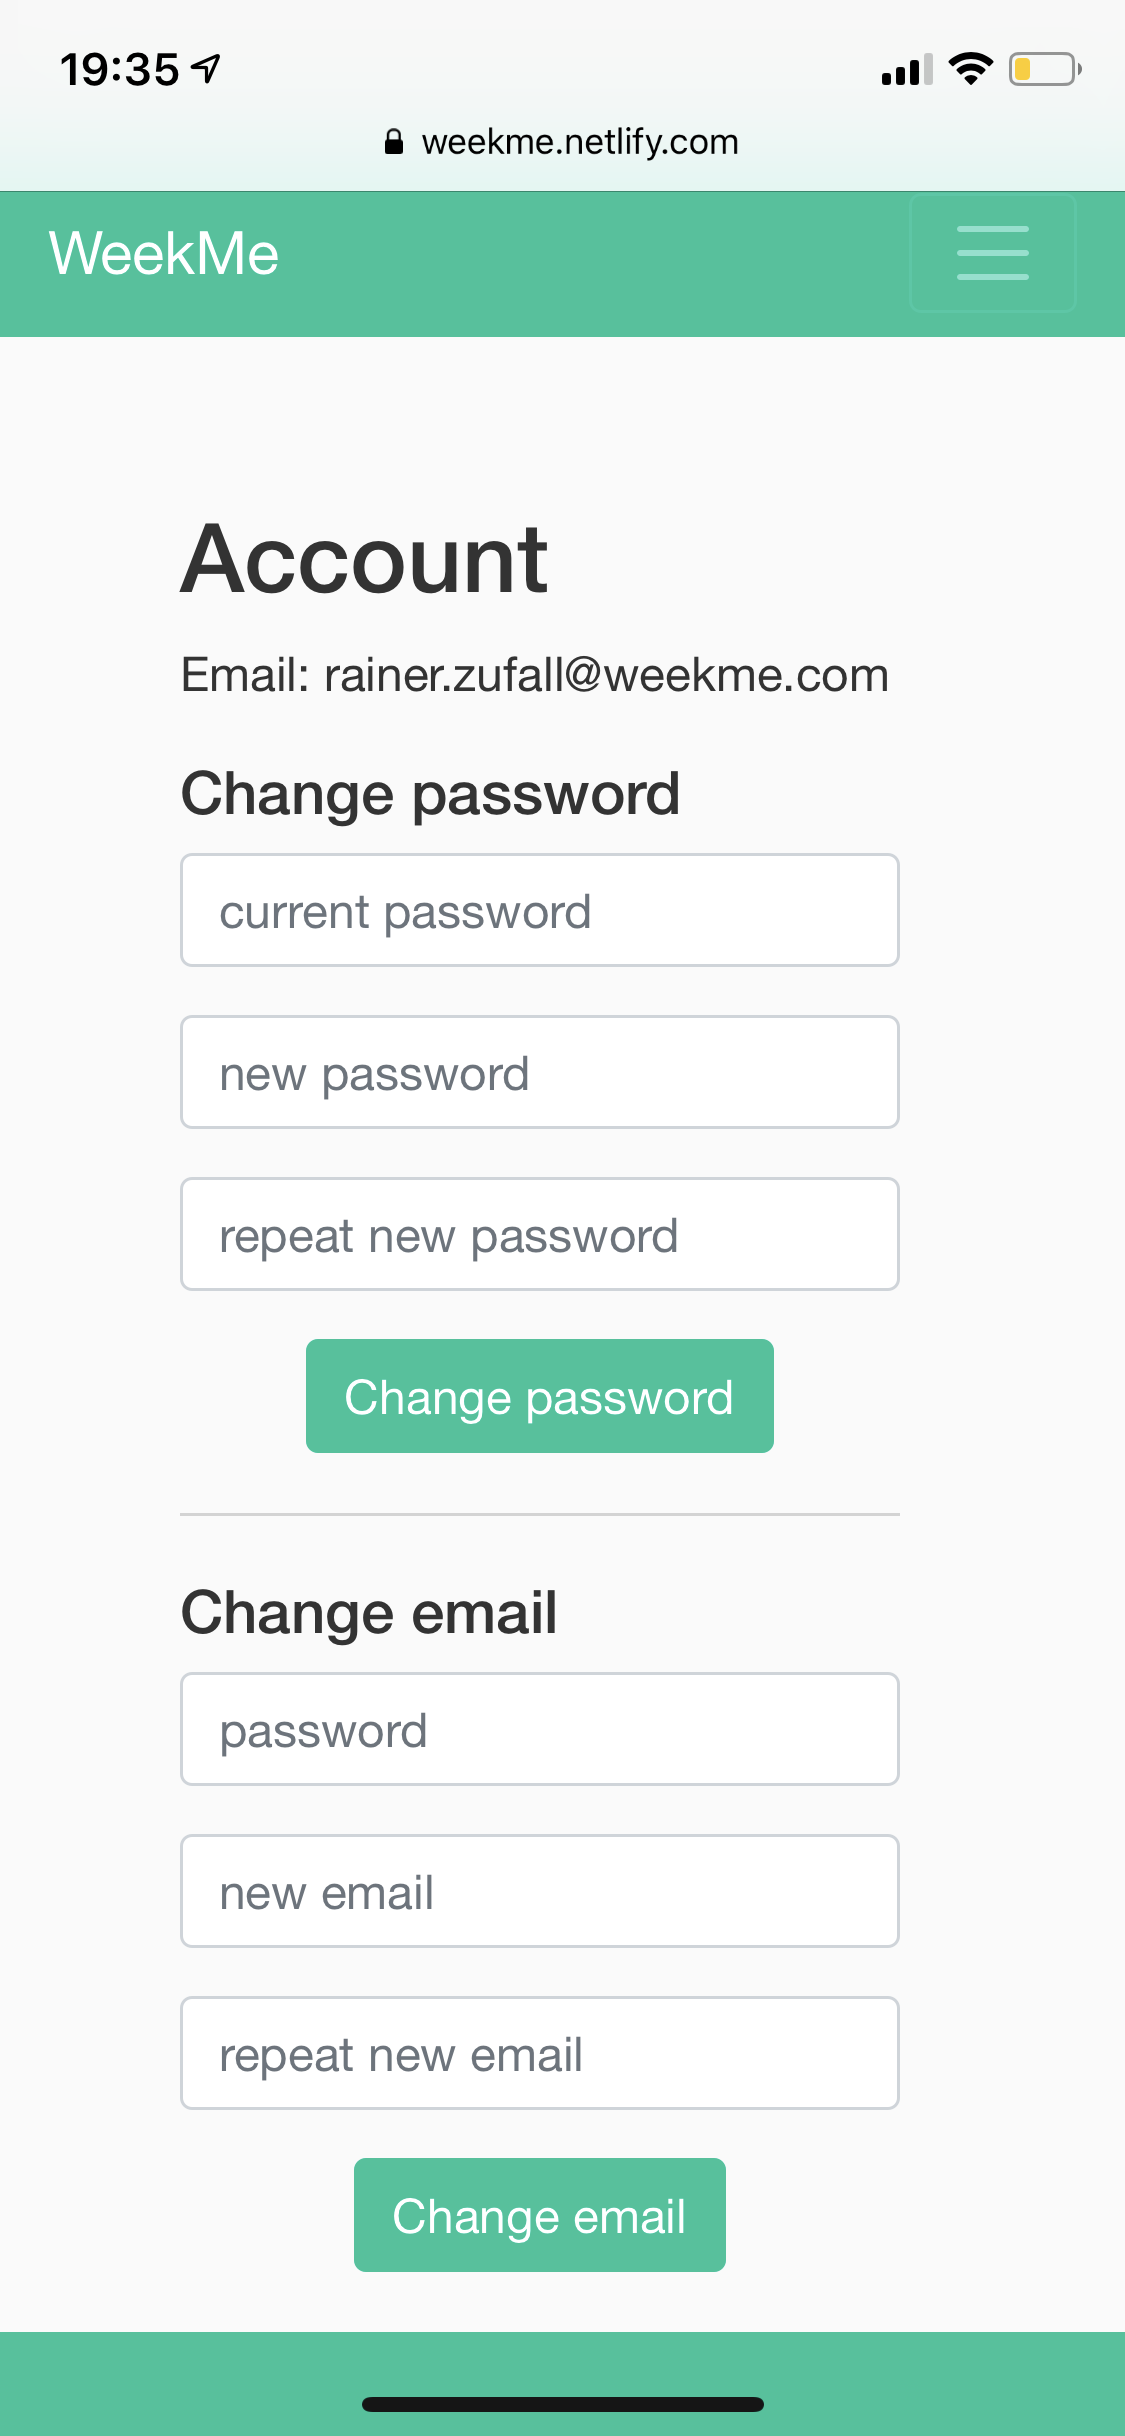
\includegraphics[height=10cm]{figures/user_docu_accounts_page.PNG}   
	\caption[WeekMe account page]{WeekMe account page on an iPhone XS}       
	\label{fig: Setting an environment variable in Heroku}     
\end{figure}  

\subsection{Working with tasks}
Since the app is all about planing your next weeks task, let's show you how you can work with these tasks on WeekMe. 
\subsubsection{Creating tasks}
To create a new task you select the plus icon where you want to add the task. This will bring up a popup window where you can enter a short description (up to 80 characters). 
If you fancy selecting a colour for your task to help you categorise, prioritise or just because you want more colour in your life - no false modesty, go on. Do it. 
In case you changed your mind or just clicked the wrong add button you can also change the day the task will be added to. 

\begin{figure}%
    \centering
    \subfloat[Popup to enter description in]{{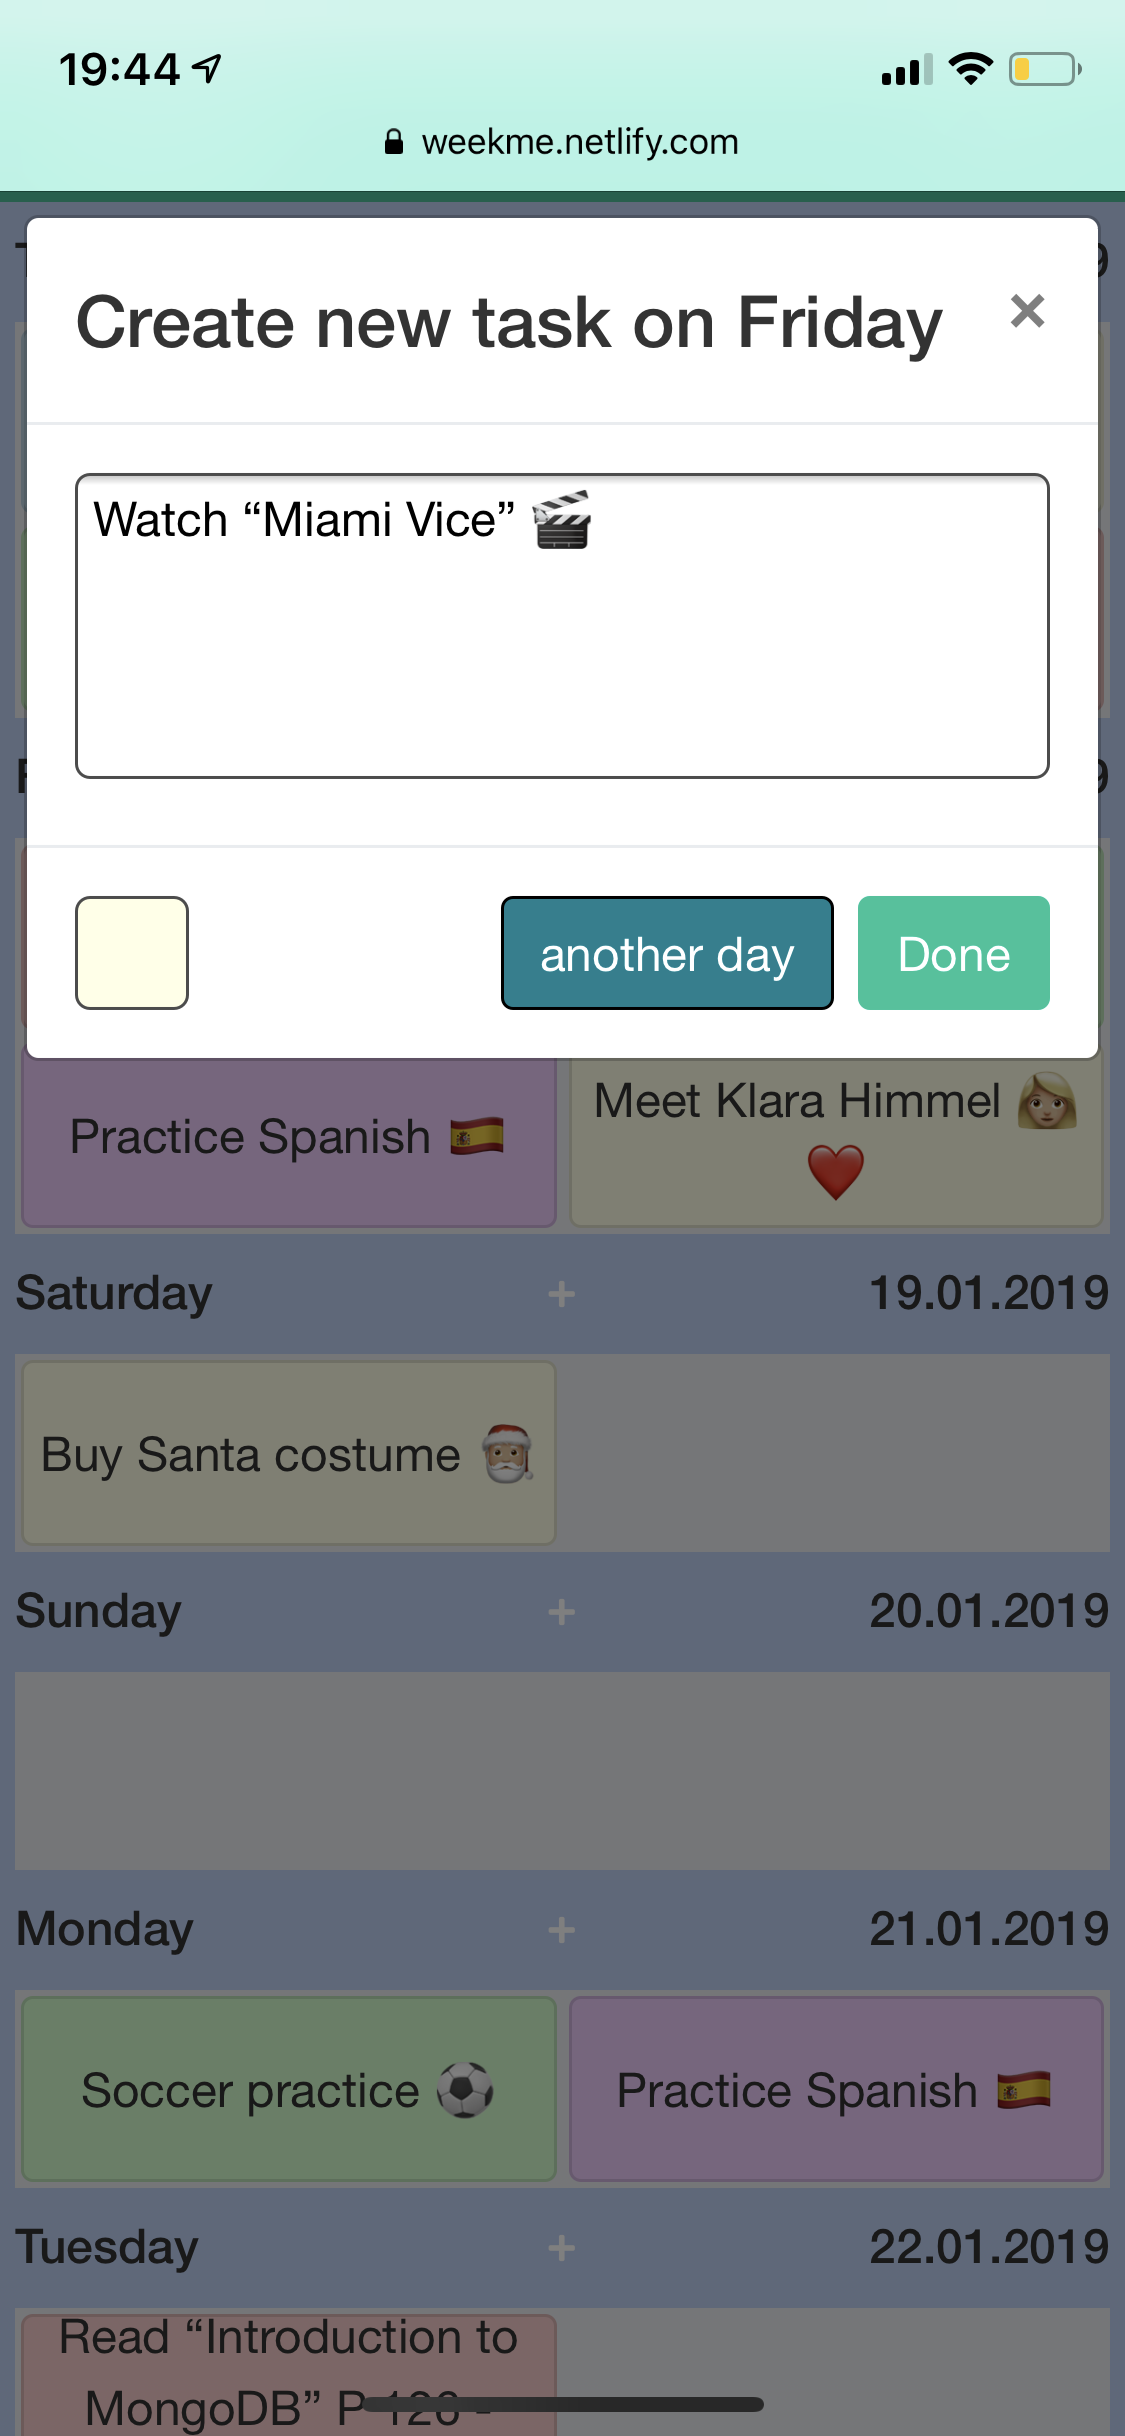
\includegraphics[height=10cm]{figures/user_docu_createtask.PNG} }}
    \qquad
    \subfloat[Change day later on]{{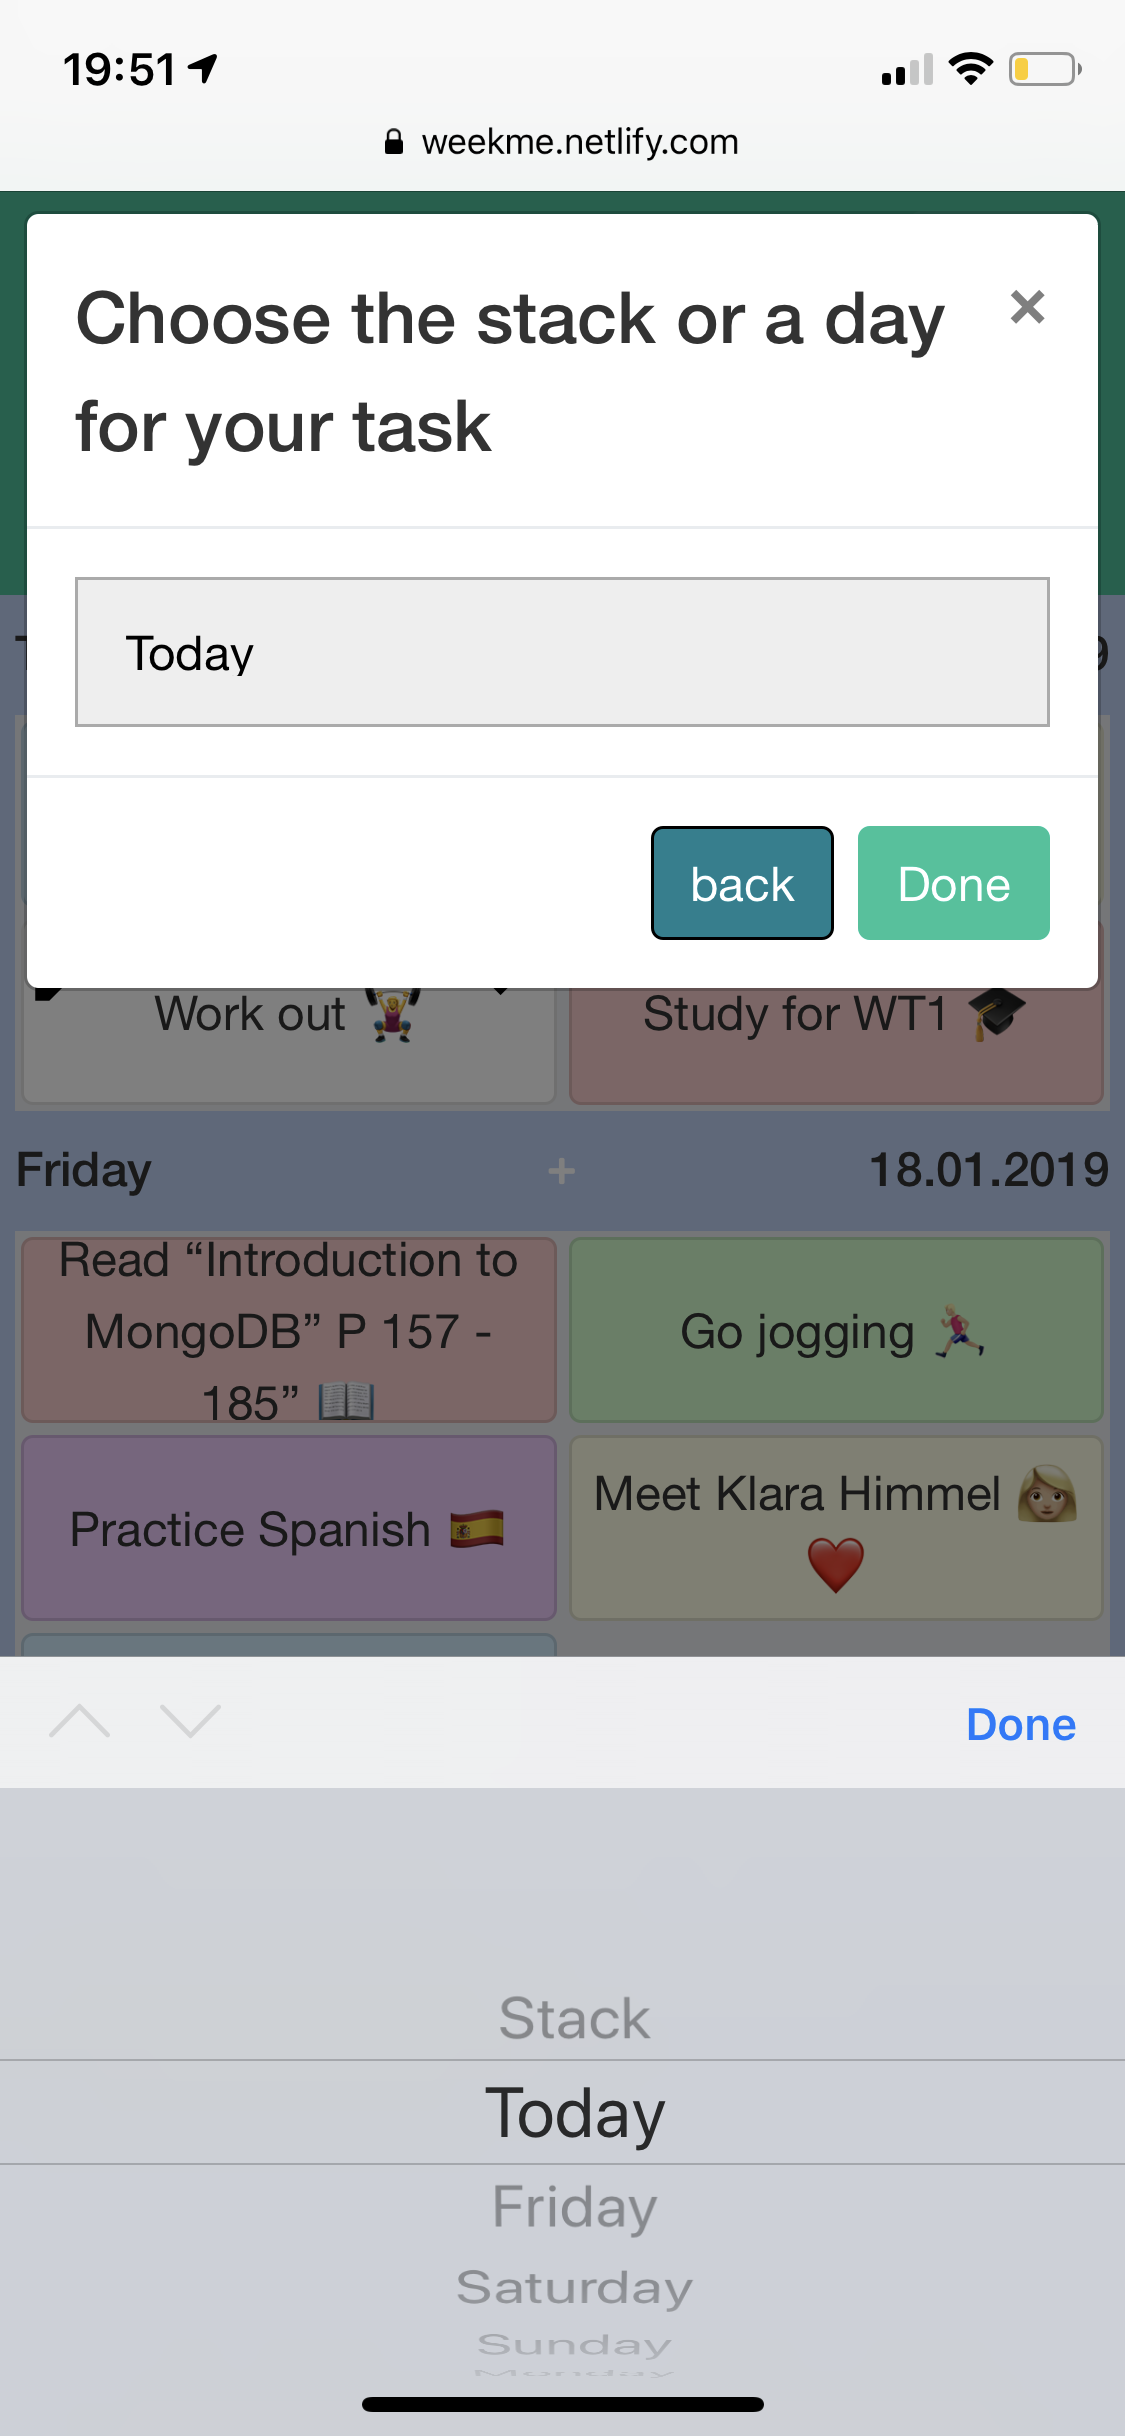
\includegraphics[height=10cm]{figures/user_docu_createtask_day.PNG} }}
    \caption{Creation process on mobile}
    \label{fig:example}
\end{figure}
 
\subsubsection{Editing tasks}

\subsubsection{Moving tasks}
\subsubsection{Deleting tasks}
\subsubsection{The stack}